\documentclass[9pt]{beamer}

\usetheme{Pittsburgh}

\usepackage[utf8]{inputenc}
\usepackage[french]{babel}
\usepackage[T1]{fontenc}
\usepackage{amsmath}
\usepackage{amsfonts}
\usepackage{amssymb}
\usepackage{graphicx}
\usepackage{hyperref}
\usepackage{url}
\usepackage{tikz}
\usepackage{tabularx}

\author[Hocine]{Alexia HOCINE\\Étudiante en Master 2 en Physique SUBAtomique}

\title{
	%Comparaison des prédictions des suites logicielles de ILC (iLCSoft) et de FCC (key4HEP) \\
	%sur un signal $ e^{+} e^{-} \longrightarrow Z H $ 
    Détecteur SDHCAL pour le signal $ e^{+} e^{-} \longrightarrow \nu \nu H $: \\
    Optimisation et Adaptation de l'analyse de données \\
    pour le Projet FCC
}
\subtitle{Superviseur : Gérald \textsc{Grenier} (IP2I équipe CMS, FCC, SDHCAL)}

\titlegraphic{
	
\includegraphics[width=0.18\textwidth]{../img/UdL-logo.png}
    \hspace{5cm}
    
\includegraphics[width=0.15\textwidth]{../img/Logo_IP2I.png}
}

\setbeamercovered{transparent} 
\setbeamertemplate{navigation symbols}{} 
\logo{} 
\institute[UCBL]{Université de Claude Bernard Lyon 1} 
\date[2022]{1\ier Juillet 2022} 
\subject{nnhA} 

% Décompte des pages sans les annexes
\setbeamertemplate{caption}[numbered]

\newcommand{\backupbegin}{
   \newcounter{framenumberappendix}
   \setcounter{framenumberappendix}{\value{framenumber}}
}

\newcommand{\backupend}{
   \addtocounter{framenumberappendix}{-\value{framenumber}}
   \addtocounter{framenumber}{\value{framenumberappendix}} 
}


% math 
\newcommand{\bbar}{\overline{b}}

\begin{document}

%%%%%%%%%%%%%%%%%%%%%%%%%%%%%%%%%%%%%%%%%%%%%%%%%%%%%%%%%%%%%%%%%%%%%%%%%%%%%%

\begin{frame}
	\titlepage
\end{frame}

%%%%%%%%%%%%%%%%%%%%%%%%%%%%%%%%%%%%%%%%%%%%%%%%%%%%%%%%%%%%%%%%%%%%%%%%%%%%%%

\begin{frame}{Sommaire}
    
    \begin{columns}
        \begin{column}{0.4\textwidth}
        \tableofcontents
        \end{column}
        \begin{column}{0.6\textwidth}
    \begin{figure}[h!]
	\center
    \resizebox{\textwidth}{!}{
	\begin{tikzpicture}%[width=\textwidth]
	
		\tikzstyle{home}=[draw, rectangle, fill=red!50, text=black, rounded corners=3pt]		
	
		\tikzstyle{directory}=[draw, rectangle, fill=gray!30, text=black, rounded corners=3pt]

		\node[directory] (A) at (0,0) {\texttt{nnhAnalysis}};
		
		\node[directory] (S) at (-4.5,-1.5) {\texttt{nnhScript}};
		\node[directory] (P) at (-1.5,-1.5) {\texttt{nnhProgram}};
		\node[directory] (R) at ( 1.5,-1.5) {\texttt{nnhResult}};
		\node[directory] (T) at ( 4.5,-1.5) {\texttt{nnhTest}};
		
		\node[home] (O) at (-4,-3) {\texttt{original}};
		\node[home] (I) at (-1.5,-3) {\texttt{ilcsoft}};
		\node[home] (F) at ( 1,-3) {\texttt{fcc}};
		
		\tikzstyle{linkDir}=[->,dotted,very thick,>=latex]
		
		\draw[linkDir] (A)--(P);
		\draw[linkDir] (A)--(R); 
		\draw[linkDir] (A)--(S);
		\draw[linkDir] (A)--(T); 
		
		\draw[linkDir] (P)--(O);
		\draw[linkDir] (P)--(I); 
		\draw[linkDir] (P)--(F);
		
	\end{tikzpicture}
    }
	\caption{
		Organisation des dossiers de mon Projet - \url{https://github.com/alexhxia/nnhAnalysis}
	}
	\label{orga:end}
\end{figure}

    \end{column}
    \end{columns}
\end{frame}

%%%%%%%%%%%%%%%%%%%%%%%%%%%%%%%%%%%%%%%%%%%%%%%%%%%%%%%%%%%%%%%%%%%%%%%%%%%%%%
\section{Introduction}
\subsection{Processus étudiés}
\begin{frame}{Introduction}

	$$ e^{+} e^{-} \longrightarrow \nu \nu h $$

	\begin{columns}
		
		\begin{column}{0.5\textwidth}
			\begin{description}
				\item[$e^{+} e^{-}$] collisionneur leptonique
				\item[$\nu \nu h$] 2 neutrinos-higgs
			\end{description}
		\end{column}
		
		\begin{column}{0.35\textwidth}
			\begin{block}{Canaux analysés}
				\begin{enumerate}
					\item $h \longrightarrow WW \longrightarrow qqqq$
					\item $h \longrightarrow b\bbar$
				\end{enumerate}
			\end{block}
        \end{column}
		
		\begin{column}{0.15\textwidth}
            \begin{block}{Mesures}
                \begin{enumerate}
                    \item 4 jets
                    \item 2 jets
                \end{enumerate}
            \end{block}
		\end{column}
	\end{columns}
    
\end{frame}

%%%%%%%%%%%%%%%%%%%%%%%%%%%%%%%%%%%%%%%%%%%%%%%%%%%%%%%%%%%%%%%%%%%%%%%%%%%%%%

\subsection{Projets de Détecteurs}
\begin{frame}{Projets iLC et FCC}{Des frabriques à bosons de Higgs}

    \begin{block}{ILC - Internationnal Linear Collider (Japon)}
        \begin{columns}
		
            \begin{column}{0.45\textwidth}
                    \begin{figure}
                        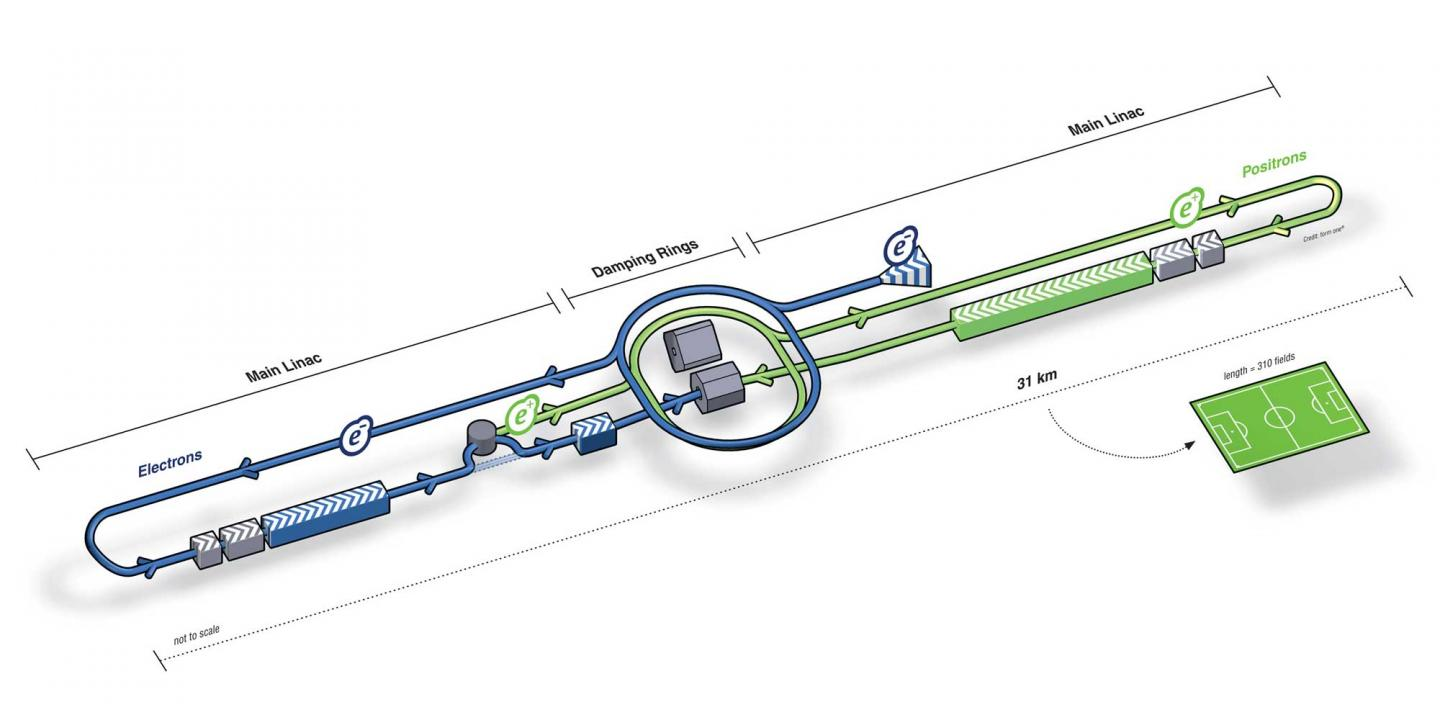
\includegraphics[width=\textwidth]{../img/ilc.jpg}
                    \end{figure}
            \end{column}
        
            \begin{column}{0.45\textwidth}
                    \begin{itemize}
                    \item Collisionneur linéaire 
                    \item 31 km (agrandissable)
                    \item 500 GeV en centre de masse
                \end{itemize}
            \end{column}
        
        \end{columns}
    \end{block}
    
    \begin{block}{FCC-ee - Future Circular Collider (CERN)}
        \begin{columns}
        
            \begin{column}{0.45\textwidth}
                \begin{figure}
                    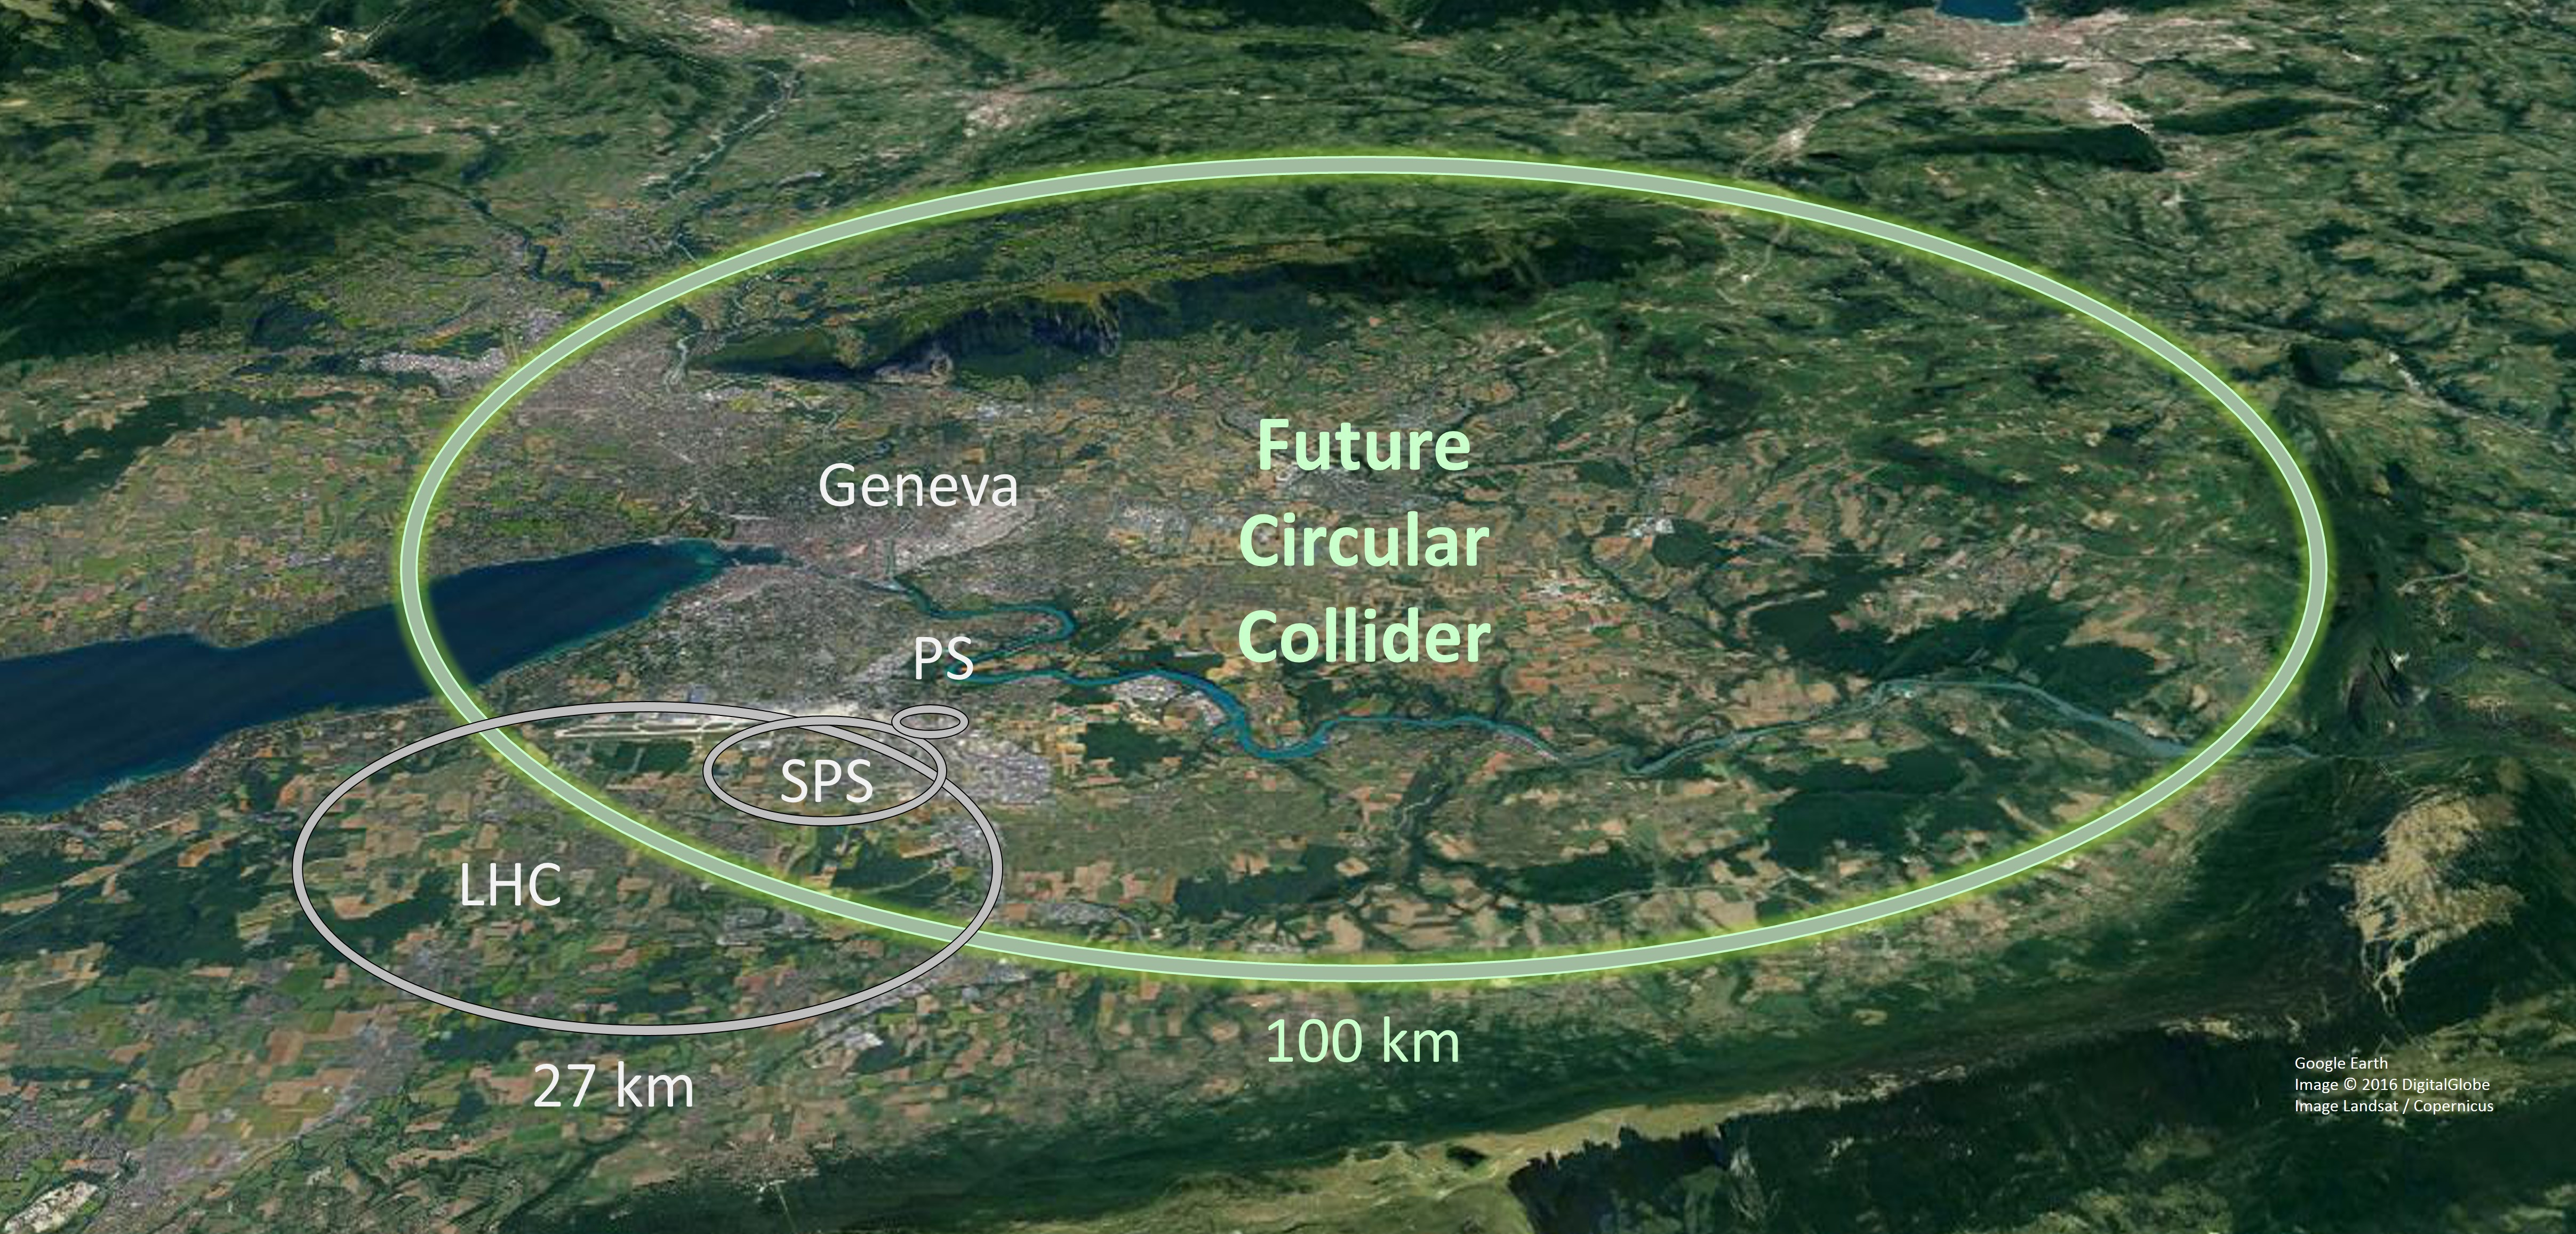
\includegraphics[width=\textwidth]{../img/FCC.jpg}
                \end{figure}
            \end{column}
            
            \begin{column}{0.45\textwidth}
                \begin{itemize}
                    \item Collisionneur circulaire
                    \item 100 km
                    \item 140 GeV dans le centre de masse
                \end{itemize}
            \end{column}
            
        \end{columns}
    \end{block}
    
\end{frame}

%%%%%%%%%%%%%%%%%%%%%%%%%%%%%%%%%%%%%%%%%%%%%%%%%%%%%%%%%%%%%%%%%%%%%%%%%%%%%%

\subsection{Détecteur SDHCAL}

\begin{frame}{Détecteur SDHCAL}
    \begin{block}{SDHCAL}

        \begin{columns}
            \begin{column}{0.5\textwidth}
                \begin{itemize}
                    \item Collaboration internationale CALICE
                    \item Semi-Digital Hadronic CALorimeter
                    \item Calorimètres à grande granularité
                    \begin{itemize}
                        \item Mesure d'énergie
                        \item Mesure de trajectoire
                        
                    \end{itemize}
                    \item Très bonne performance des Algorithmes de Flux de Particules
                    \item Candidat pour les futurs collisionneurs leptoniques
                    \item Septembre nouvelle phase de tests en faisceaux
                    \item En cours de développement : exploitation du temps à 100 pico s
                \end{itemize}
            \end{column}
	
            \begin{column}{0.45\textwidth}
                \begin{figure}
                    \center
                    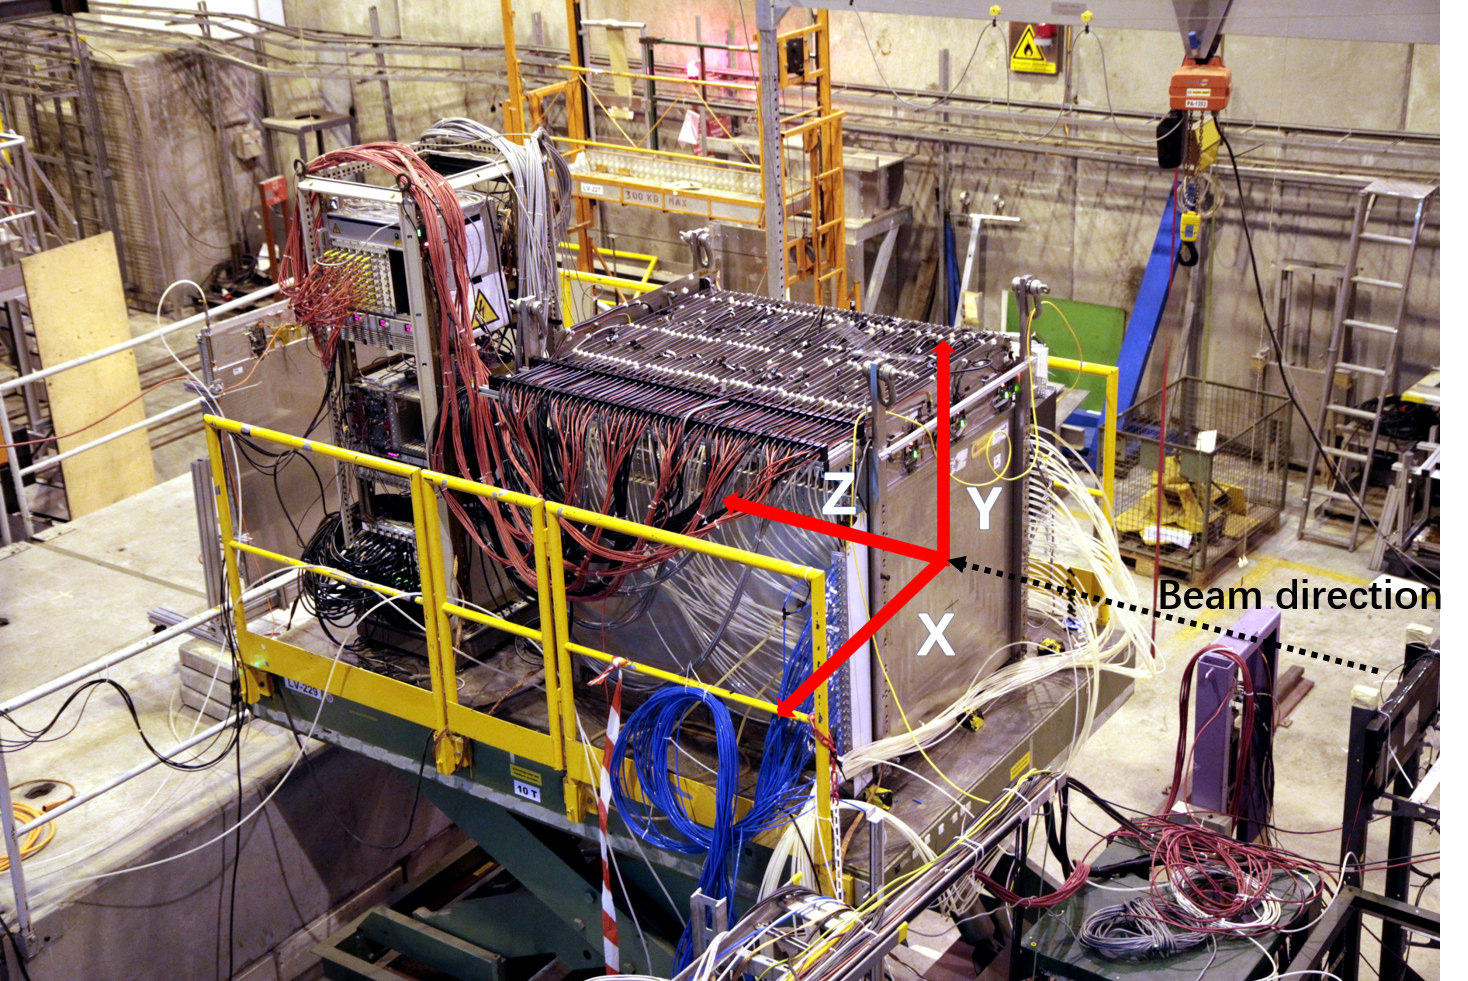
\includegraphics[width=\textwidth]{../img/SDHCAL.png}
                    \caption{Détecteur SDHCAL}
                    \label{detector}
                \end{figure}
            \end{column}
        \end{columns}
    \end{block}
\end{frame}

%%%%%%%%%%%%%%%%%%%%%%%%%%%%%%%%%%%%%%%%%%%%%%%%%%%%%%%%%%%%%%%%%%%%%%%%%%%%%%
\section{Programmes}

\subsection{original}

\begin{frame}{original}{https://github.com/alexhxia/nnhAnalysis/tree/main/nnhProgram/original}

\begin{block}{Projet initial}
	\url{https://github.com/ggarillot/nnhAnalysis/tree/refactor}
\end{block}

\begin{columns}

	\begin{column}{0.33\textwidth}
		\begin{block}{\texttt{miniDSTMaker}}
			Télécharge du server \texttt{lyogrid06} les fichiers \texttt{DST} de \texttt{DESY} : \texttt{.lcio}
		\end{block}
	\end{column}
	
	\begin{column}{0.33\textwidth}
		\begin{block}{\texttt{processor}}
			Transforme les fichiers \texttt{.lcio} en \texttt{.root} par type de processus
		\end{block}
	\end{column}
	
	\begin{column}{0.33\textwidth}
		\begin{block}{\texttt{analysis}}
			Entraine une BDT, pour obtenir l'analyse statistique des évènements
		\end{block}
	\end{column}

\end{columns}

\begin{block}{Type de processus}
	\begin{figure}
		\center
		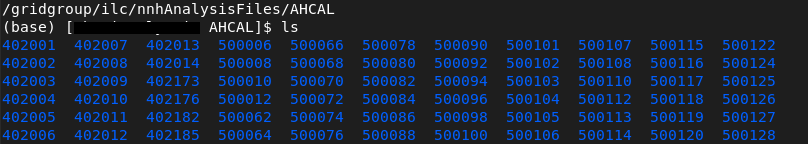
\includegraphics[width=\textwidth]{../img/listeProcessus.png} 
	\end{figure}
\end{block}

\end{frame}

%%%%%%%%%%%%%%%%%%%%%%%%%%%%%%%%%%%%%%%%%%%%%%%%%%%%%%%%%%%%%%%%%%%%%%%%%%%%%%

\begin{frame}{Principe d'une BDT}

    \begin{columns}
    
        \begin{column}{0.5\textwidth}
            \begin{block}{Boosted Decision Tree}
                \begin{itemize}
                    \item Arbres de décision boostés
                    \item Machine Learning - apprentissage automatique
                    \item Création d'un modèle, ici pour déterminer le type de processus 
                    
                \end{itemize}
            \end{block}
            \begin{alertblock}{Pour 2 exécutions à partir des mêmes données}
                \begin{itemize}
                    \item fichiers de sortie ne sont pas identiques 
                    \item mais doivent être équivalent
                \end{itemize}
            \end{alertblock}
        \end{column}
        
        \begin{column}{0.5\textwidth}
            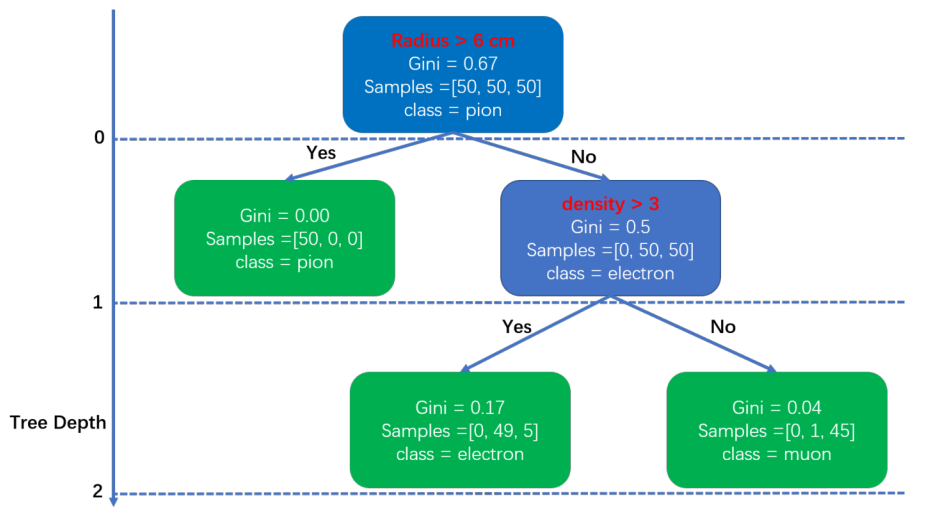
\includegraphics[width=\textwidth]{../img/ExampleBDT.png}
        \end{column}
        
    \end{columns}

\end{frame}

%%%%%%%%%%%%%%%%%%%%%%%%%%%%%%%%%%%%%%%%%%%%%%%%%%%%%%%%%%%%%%%%%%%%%%%%%%%%%%
\subsection{iLCSoft}

\begin{frame}{iLCSoft}{https://github.com/alexhxia/nnhAnalysis/tree/main/nnhProgram/ilcsoft}

	\begin{block}{Améliorations apporter à \texttt{processor} et \texttt{analysis}}
		\begin{itemize}
			\item Réécritures minimes (typographie, typage \texttt{auto})
			\item Modification des noms de certaines fonctions
			\item Ajouts de commentaires (clarification des contrats)
			\item Nouvelle classe pour simplifier l'utilisation des codes PDG : \texttt{PDGInfo.XX}\\
					\texttt{XX = \{hh, cc\}}
			\item Réorganisation de la gestion des fichiers des sortis pour permettre l'exécution en parallèle (en cours)
		\end{itemize}
	\end{block}
	
	\begin{block}{\texttt{miniDSTMaker}}
		\begin{itemize}
			\item Non pertinent pour ce stage, puisque les données sont locales
		\end{itemize}
	\end{block}

\end{frame}

%%%%%%%%%%%%%%%%%%%%%%%%%%%%%%%%%%%%%%%%%%%%%%%%%%%%%%%%%%%%%%%%%%%%%%%%%%%%%%
\subsection{FCC}

\begin{frame}{FCC}{https://github.com/alexhxia/nnhAnalysis/tree/main/nnhProgram}

	\begin{block}{Ajout du programme \texttt{convert} (en cours)}
		\begin{itemize}
			\item Tranforme les fichiers \texttt{.lcio}, exploitable par iLCSoft, en fichier exploitable par FCC.
			\item De la suite logiciel \texttt{LCIO} vers \texttt{EDM4hep}
		\end{itemize}
	\end{block}

	\begin{block}{\texttt{processor} (en cours)}
		\begin{itemize}
			\item Change toutes les utilisations de la suite logicielle d'iLCSoft vers key4HEP
		\end{itemize}
	\end{block}

	\begin{block}{\texttt{analysis}}
		\begin{itemize}
			\item Ne demande aucune nouvelle modification
		\end{itemize}
	\end{block}

\end{frame}

%%%%%%%%%%%%%%%%%%%%%%%%%%%%%%%%%%%%%%%%%%%%%%%%%%%%%%%%%%%%%%%%%%%%%%%%%%%%%%
\section{Outils Numériques}

\subsection{Script}

\begin{frame}{Outils de Numérique : \texttt{Script}}{https://github.com/alexhxia/nnhAnalysis/tree/main/nnhScript}

\begin{block}{Liste de nouveaux scripts}
	\begin{description}
		\item[\texttt{nnh}] programme général 
		\begin{itemize}
			\item permet de choisir :
			\begin{itemize}
				\item combien de programme \texttt{processus} et \texttt{analysis} on souhaite
			\end{itemize}
		\end{itemize}
		\begin{description}
			\item[\texttt{nnhProcessor}] lance un programme \texttt{processus} complet
			\item[\texttt{nnhAnalysis}] lance un programme \texttt{analysis} complet
			\begin{description}
				\item[\texttt{prepareBDT}] lance le programme \texttt{prepareBDT}
				\item[\texttt{launchBDT}] lance le programme \texttt{launchBDT}
			\end{description}
		\end{description}
	\end{description}
\end{block}

\end{frame}

%%%%%%%%%%%%%%%%%%%%%%%%%%%%%%%%%%%%%%%%%%%%%%%%%%%%%%%%%%%%%%%%%%%%%%%%%%%%%%
\subsection{Test}

\begin{frame}{Outils de Numérique : \texttt{Test}}{https://github.com/alexhxia/nnhAnalysis/tree/main/nnhTest}

\begin{block}{Programme de tests : \texttt{testXxYy.py}}
	\begin{itemize}
		\item Teste grâce à le fonction de Kolmogorov - développé par ROOT (CERN)
		\item Teste les fichiers de sortis :
		\begin{itemize}
			\item des programmes \texttt{Xx = \{processus, analysis\}}
			\item de type \texttt{Yy = \{Completed, Same\}}
		\end{itemize}
	\end{itemize}
	\begin{tabular}{| c | c | c |}
		\hline
			\texttt{•} & \texttt{Processus} & \texttt{Analysis} \\
		\hline
			\texttt{Completed} & \texttt{testProcessorCompleted.py} & \texttt{testAnalysisCompleted.py} \\
		\hline
			\texttt{Same} & \texttt{testProcessorSame.py} & \texttt{testAnalysisSame.py} \\
		\hline
	\end{tabular}
	\begin{description}
		\item[\texttt{Completed}] teste si tous les fichiers ont bien été généré
		\item[\texttt{Same}]	teste les différences entre 2 séries de fichiers
		\begin{description}
			\item[\texttt{processus}] tous les fichiers sont sensés être identiques
			\item[\texttt{analysis}] certains les fichiers sont sensés :
            \begin{itemize}
                \item être identiques : \texttt{DATA.root}, données initiales 
                \item d'autres différents : \texttt{model\_[...].root}
                \item d'autres équivalents : \texttt{stats\_[...].root} 
            \end{itemize}
		\end{description}
	\end{description}
\end{block}

\end{frame}

%%%%%%%%%%%%%%%%%%%%%%%%%%%%%%%%%%%%%%%%%%%%%%%%%%%%%%%%%%%%%%%%%%%%%%%%%%%%%%
\section{Conclusion}

\begin{frame}{Conclusion}

\begin{columns}

	\begin{column}{0.45\textwidth}
		\begin{exampleblock}{Travails réalisés}
			\begin{itemize}
		 		\item Optimisation des codes pour iLCSoft \texttt{processor}
		 		\item Automatisation des programmes
		 		\item Programmation de codes de test
			\end{itemize}
		\end{exampleblock}
        \begin{alertblock}{Travails en cours}
			\begin{itemize}
		 		\item Optimisation des codes pour iLCSoft \texttt{analysis}
		 		\item Adaptation au projet FCC
			\end{itemize}
		\end{alertblock}
	\end{column}
	
    %\pause
	\begin{column}{0.45\textwidth}
		\begin{block}{Compétences renforcées}
			\begin{itemize}
                \item Programmation
                \begin{itemize}
                    \item C++
                    \item ROOT
                    \item Python
                    \item Script bash
                \end{itemize}
                
                \item Physique
                \begin{itemize}
                    \item Physique des Particules
                    \item Modèle Standard
                    \item Statistiques
                \end{itemize}
            
			\end{itemize}
		\end{block}
        
        \begin{exampleblock}{Nouvelles compétences}
			\begin{itemize}
		 		\item Utilisation de BDT
			\end{itemize}
		\end{exampleblock}
        
	\end{column}

\end{columns}

\end{frame}

%%%%%%%%%%%%%%%%%%%%%%%%%%%%%%%%%%%%%%%%%%%%%%%%%%%%%%%%%%%%%%%%%%%%%%%%%%%%%%
\backupbegin
%%%%%%%%%%%%%%%%%%%%%%%%%%%%%%%%%%%%%%%%%%%%%%%%%%%%%%%%%%%%%%%%%%%%%%%%%%%%%%

\begin{frame}{Sources des Figures}

\listoftables 

%\begin{description}
	%\item[\ref{fig:Michelson}] \url{public.virgo-gw.eu/index.php?gmedia=Rv7bB&t=g\#photoBox-54}
%\end{description}

\end{frame}

%%%%%%%%%%%%%%%%%%%%%%%%%%%%%%%%%%%%%%%%%%%%%%%%%%%%%%%%%%%%%%%%%%%%%%%%%%%%%%

\begin{frame}{Bibliographie}

%\begin{description}
	%\item[\ref{fig:Michelson}] \url{public.virgo-gw.eu/index.php?gmedia=Rv7bB&t=g\#photoBox-54}
%\end{description}

\end{frame}

%%%%%%%%%%%%%%%%%%%%%%%%%%%%%%%%%%%%%%%%%%%%%%%%%%%%%%%%%%%%%%%%%%%%%%%%%%%%%%
\appendix
\begin{frame}

\begin{center}
\Huge{Suppléments}
\end{center}

\end{frame}

%%%%%%%%%%%%%%%%%%%%%%%%%%%%%%%%%%%%%%%%%%%%%%%%%%%%%%%%%%%%%%%%%%%%%%%%%%%%%%

\begin{frame}{Annexes}
\end{frame}

%%%%%%%%%%%%%%%%%%%%%%%%%%%%%%%%%%%%%%%%%%%%%%%%%%%%%%%%%%%%%%%%%%%%%%%%%%%%%%
\backupend
\end{document}
